\documentclass{beamer}

% Must be loaded first
\usepackage{tikz}

\usepackage[utf8]{inputenc}
\usepackage{textpos}

% Font configuration
\usepackage{fontspec}

\input{font.tex}

% Tikz for beautiful drawings
\usetikzlibrary{mindmap,backgrounds}
\usetikzlibrary{arrows.meta,arrows}
\usetikzlibrary{shapes.geometric}

% Minted configuration for source code highlighting
\usepackage{minted}
\setminted{highlightcolor=black!5, linenos}
\setminted{style=perldoc}

\usepackage[listings, minted]{tcolorbox}
\tcbset{left=6mm}

% Use the include theme
\usetheme{codecentric}

% Metadata
\title{How This Presentation Was Made}
\author{Markus Hauck @markus1189}

\newcommand{\recipe}{%
  \begin{itemize}
  \item AST
  \item \texttt{inject}
  \item interpreter
  \item check laws
  \end{itemize}
}

% The presentation content
\begin{document}

\begin{frame}[noframenumbering,plain]
  \titlepage{}
\end{frame}

\section{Introduction}\label{sec:introduction}

\begin{frame}
  \frametitle{Presentations}
  \begin{center}
    \includegraphics[width=\textwidth]{ditaa/presentations.png}
  \end{center}
\end{frame}

\begin{frame}
  \frametitle{Presentations: But How}
  \begin{itemize}
  \item powerpoint/keynote/google slides/\ldots{}
  \item but you can't use \texttt{git} :(
  \item requirement: some markup language-ish thing
  \item e.g., pandoc / LaTeX
  \item text handled, what about pictures/code/etc?
  \end{itemize}
\end{frame}

\begin{frame}
  \frametitle{How It All Started}
  \begin{itemize}
  \item Me writing presentation be like:
  \item fighting graphical editor more than focused on content
  \item logical step: switch to something that is text based
  \item how to handle generated pictures
  \item how to handle code
  \end{itemize}
\end{frame}

\begin{frame}
  \frametitle{Writing Presentation}
  \begin{itemize}
  \item quick and dirty: google slides, powerpoint, keynote
  \item can't use version control like git
  \item paste pictures
  \item want to change something? awful
  \end{itemize}
\end{frame}

\begin{frame}
  \frametitle{Used Tools}
  \begin{itemize}
  \item Nix for system dependencies + build env
  \item Shake to write a custom build system
  \item Dhall for easy configuration
  \item LaTeX for slides
  \item ditaa, graphviz
  \item more...
  \end{itemize}
\end{frame}

\begin{frame}
  \frametitle{Presentations}
  \begin{itemize}
  \item having CI would be nice :thinking:
  \item ``just'' check out from github and build it?
  \item good luck with that!
  \end{itemize}
\end{frame}

\begin{frame}
  \frametitle{Pain Points}
  \begin{itemize}
  \item you have to setup LaTeX
  \item plus all required packages (most of the time: \textbf{all})
  \item hope that everything is up to date and try to build it
  \item notice missing fonts, try to find them somewhere
  \item notice missing python package (pygments), install it
  \item lots of trial and error \texttt{:(}
  \end{itemize}
\end{frame}

\begin{frame}
  \frametitle{Continuous Integration via Travis}
  \inputminted[linenos=false, fontsize=\tiny, lastline=31]{yaml}{static-source/long-travis-ci.yml}
\end{frame}

\begin{frame}
  \frametitle{Continuous Integration via Travis}
  \inputminted[linenos=false, fontsize=\tiny, firstline=31, lastline=60]{yaml}{static-source/long-travis-ci.yml}
\end{frame}

\begin{frame}
  \frametitle{Continuous Integration via Travis}
  \inputminted[linenos=false, fontsize=\tiny, firstline=61, lastline=90]{yaml}{static-source/long-travis-ci.yml}
\end{frame}

\begin{frame}
  \frametitle{Continuous Integration via Travis}
  \inputminted[linenos=false, fontsize=\tiny, firstline=91, lastline=120]{yaml}{static-source/long-travis-ci.yml}
\end{frame}

\begin{frame}
  \frametitle{Presentation As Code}
  \begin{itemize}
  \item reproducible: same description for CI and local machine
  \item single step: one command
  \item declarative: generate from description
  \item checked: source code compiles
  \end{itemize}
\end{frame}

\begin{frame}
  \frametitle{Scenarios}
  \begin{itemize}
  \item Nix, Shake and Dhall
  \item Scenario 1: Dependencies
  \item Scenario 2a: Editing Code
  \item Scenario 2b: Checking Snippets
  \item Scenario 3: Generated Pictures
  \item Scenario 4: Continuous Integration
  \end{itemize}
\end{frame}

\section{Shake}

\begin{frame}
  \frametitle{Shake}
  \begin{itemize}
  \item \url{shakebuild.com/manual}
  \item Shake is a Haskell \textbf{library} for writing build systems
  \item \texttt{Shake} vs \texttt{make} is like \texttt{Monad} vs \texttt{Applicative}
  \item integrates well with other libraries and system tools
  \item the backbone of this presentation
  \end{itemize}
\end{frame}

\begin{frame}
  \frametitle{Shake}
  \begin{itemize}
  \item specify rules to create output from some input
  \item avoid rebuilds of unchanged things
  \item ``just'' a library, rest is up to you
  \end{itemize}
\end{frame}

\begin{frame}[fragile]
  \frametitle{Shake Rules}
  \begin{minted}{haskell}
--  +---------------- file pattern to match
--  |
--  |       +-------- target path to create
--  |       |
--  v       v
pattern %> \out -> do
  action1          -- <--\
  action2          -- <---+- Actions to build 'out'
  action3          -- <--/
  \end{minted}
\end{frame}

\begin{frame}[fragile]
  \frametitle{Shake Rules}
  \begin{minted}{haskell}
"*.txt" %> \out -> do
  putNormal "Debug"
  cmd "touch" [out]
  \end{minted}
\end{frame}

\begin{frame}[fragile]
  \frametitle{Shake Rules}
  \inputminted[autogobble]{haskell}{snippets/pdf-rule.hs}
\end{frame}

\begin{frame}
  \frametitle{Shake Rules}
  \begin{center}
    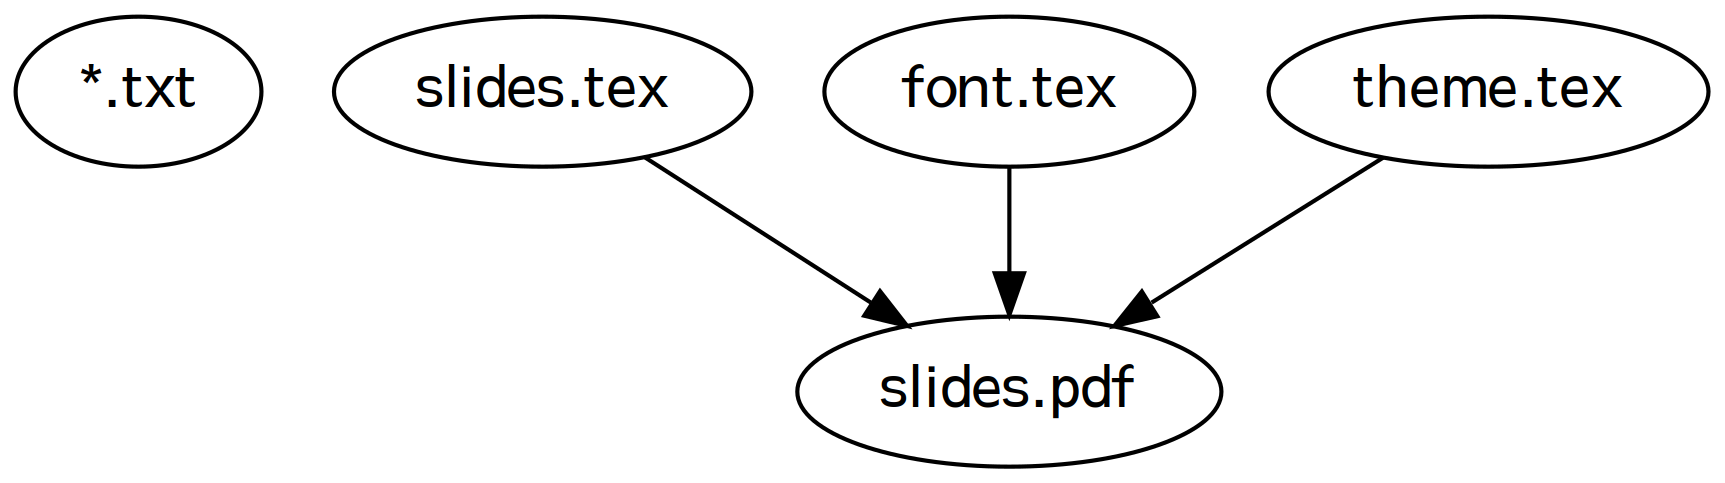
\includegraphics[width=0.8\textwidth]{graphviz/rules.png}
  \end{center}
\end{frame}

\begin{frame}
  \frametitle{Editing Code}
  \begin{itemize}
  \item Step 1: Implement your code in a Scala project
  \item Step 2: Wild Copy And Paste Into Presentation
  \item Step 3: Reformat To Fit Slide
  \item Step 4: Change Original Source Code
  \item Step 5: Wild Editing Of Code on Slides
  \item Step 6: Being suspicious that something is broken (optional)
  \end{itemize}
\end{frame}

\begin{frame}[fragile]
  \frametitle{Extract Code}
  \begin{itemize}
  \item common: extract based on lines
  \item after edit / formatting / \ldots they change
  \item not what we want
  \end{itemize}
\end{frame}

\begin{frame}
  \frametitle{Editing Code}
  \begin{itemize}
  \item idea: extract source code directly from actual project
  \item use comments to delimit ``snippets''
  \item write code to extract everything in between
  \end{itemize}
\end{frame}

\begin{frame}
  \frametitle{Editing Code}
  \begin{itemize}
  \item add comments in the code
  \item write a small ``snippet'' file
  \item let shake automatically extract snippets
  \item include code snippets in presentation
  \end{itemize}
\end{frame}

\begin{frame}
  \frametitle{Annotating Code for Snippets (META)}
  \inputminted[autogobble]{haskell}{snippets/outer-pdf-rule.hs}
\end{frame}

\begin{frame}
  \frametitle{Snippet File}
  \inputminted{text}{snippets/pdf-rule.snippet}
\end{frame}

\begin{frame}
  \frametitle{Extracting Code}
  \begin{itemize}
  \item don't want to litter your source?
  \item as long as search pattern is unique, no problem
  \item will always be up to date with the compiling source
  \item but we also have to format and maybe check again
  \end{itemize}
\end{frame}

\begin{frame}
  \frametitle{Editing Code}
  \begin{itemize}
  \item let's tackle checking first
  \item lots of times: broken code snippets that never compile
  \item mostly hand waving examples
  \item style errors you would notice in your actual setup
  \item wouldn't it be cool to get that for your presentation
  \end{itemize}
\end{frame}

\begin{frame}
  \frametitle{Checking Code}
  \begin{itemize}
  \item after extracting a snippet into an includable file
  \item run linter/compiler/...
  \item fail building presentation if the command fails
  \end{itemize}
\end{frame}

\begin{frame}
  \frametitle{Formatting Code}
  \begin{itemize}
  \item just another step like linting
  \item run formatter of choice on the source file
  \item e.g. format to a width of 55 chars
  \end{itemize}
\end{frame}

\begin{frame}
  \frametitle{Formatting Code}
  \begin{itemize}
  \item example of code:
  \end{itemize}
\end{frame}

\begin{frame}
  \frametitle{Pictures}
  \begin{itemize}
  \item need more pictures
  \item downloaded, but from where?
  \item maybe needs conversion and scaling
  \item commit them to the repository?
  \item generated by an external tool (ditaa, plantuml, graphviz, ...)
  \item we'll tackle both
  \end{itemize}
\end{frame}

\begin{frame}
  \frametitle{Downloading Pictures}
  \begin{itemize}
  \item write a new Shake rule of course
  \item normal download of the file from the internet
  \item provide a file per image that contains url + imagemagick instructions
  \item the rule in Haskell: code
  \end{itemize}
\end{frame}

\begin{frame}
  \frametitle{Downloading Pictures}
  \includegraphics{images/maintain-make.jpg}
\end{frame}

\begin{frame}
  \frametitle{Generating Pictures}
  \begin{itemize}
  \item common scenario: picture is generated
  \item there is a file that describes it + tool to render
  \item Steps:
    \begin{itemize}
    \item write the description file
    \item generate graphic
    \item include in presentation
    \item notice change needed :(
    \end{itemize}
  \end{itemize}
\end{frame}

\begin{frame}
  \frametitle{Dhall For Configuration?}
  \begin{itemize}
  \item what is Dhall
  \item why Dhall
  \end{itemize}
\end{frame}

\begin{frame}
  \frametitle{Generating Pictures}
  \begin{itemize}
  \item the description: Dhall
  \item check if already downloaded
  \item download
  \item apply imagemagick transformation
  \end{itemize}
\end{frame}

\begin{frame}
  \frametitle{The One Command Lie}
  \begin{itemize}
  \item you just have to run this \textbf{one} command
  \item it's mostly a lie
  \item with nix, you can \textit{actually} achieve that!
  \item perfect: use it in .travis.yml as well as every pc
  \end{itemize}
\end{frame}

\section{Conclusion}\label{sec:conclusion}

\begin{frame}
  \begin{center}
    \Huge
    Thanks for your attention
  \end{center}
  \begin{center}
    \Huge
    Markus Hauck (@markus1189)
  \end{center}
\end{frame}

\begin{frame}
  \tableofcontents{}
\end{frame}

\appendix{}

\section*{Bonus}\label{sec:bonus}

\end{document}
